\section{M-DocSum-Bench}

\begin{table}[tbp]
\caption{Overall Statistics of M-DocSum-Bench. This includes the number of documents (Docs), the average number of text tokens (Tokens), and an indicator of whether the documents are multi-page (Multi). The evaluated model capabilities are denoted by U, R, L, S, representing Understanding, Reasoning, Locating, and Summarization, respectively. Data types are classified as Synthetic (generated data), Realistic (purely manually annotated data), and Hybrid (a mix of synthetic and realistic data).}

\centering
\resizebox{0.47\textwidth}{!}{
\begin{tabular}{lcccccccc}
\toprule
Benchmarks & Docs & Tokens & Multi & U & R & L & S & Type \\
\midrule
DocVQA        & -       & 151.5   & $\times$          & $\checkmark$   & $\times$   & $\times$  & $\times$        & synthetic          \\
ChartQA       & -       & 236.9   & $\times$          & $\checkmark$   & $\times$   & $\times$  & $\times$        & synthetic         \\
RULER & any       & any   & $\checkmark$     & $\checkmark$   & $\times$  & $\times$     & $\times$  & synthetic          \\
DUDE & 5019    & 1,831.5 & $\checkmark$     & $\checkmark$   & $\checkmark$   & $\times$  & $\times$   & hybrid          \\
loong  & 1600    & 110,900 & $\checkmark$     & $\checkmark$   & $\checkmark$     & $\times$  & $\times$      & hybrid     \\
MMLongBench  & 135     & 21,214.1 & $\checkmark$    & $\checkmark$      & $\checkmark$      & $\times$     & $\times$ & Realistic       \\
M-Longdoc & 180 & 120,988 & $\checkmark$ & $\checkmark$ & $\checkmark$ & $\times$  & $\times$ & hybrid  \\
DocBench  & 229     & 46,377 & $\checkmark$     & $\checkmark$      & $\checkmark$      & $\times$      & $\times$      & hybrid \\
LongDocURL  & 396 & 43,622.6 & $\checkmark$  & $\checkmark$ & $\checkmark$      & $\checkmark$   & $\times$  & hybrid        \\
\midrule
\textbf{M-DocSum-Bench}            & 500    & 12,912.4 & $\checkmark$   & $\checkmark$     & $\checkmark$   & $\checkmark$   & $\checkmark$  & hybrid        \\
\bottomrule
\end{tabular}
}
\label{tab:statis}
\end{table}
\begin{figure}[t]
\centering
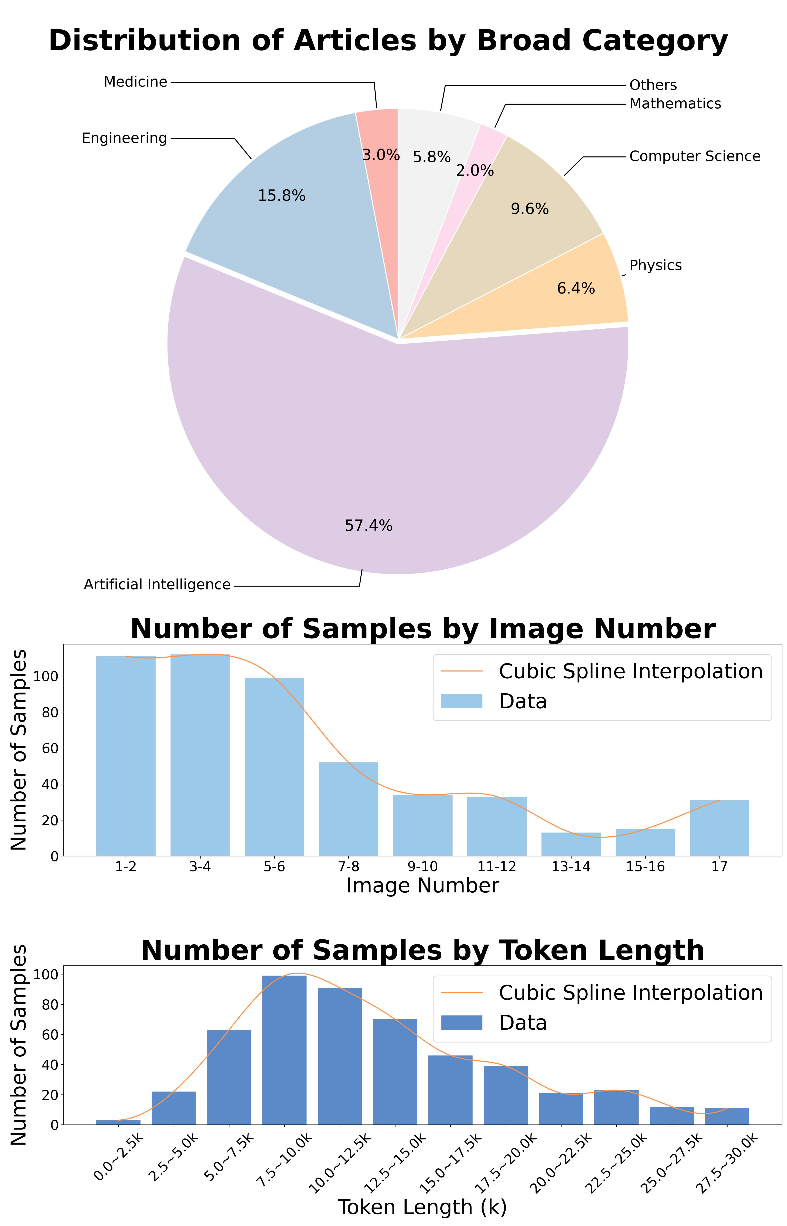
\includegraphics[width=0.47\textwidth]{figs/statis-shu}
\caption{The quantitative indicators of M-DocSum-Bench display fundamental information such as token length, image count, and document topics.}
\label{fig:1_statisticians}
\end{figure}

\begin{figure*}[t]
\centering
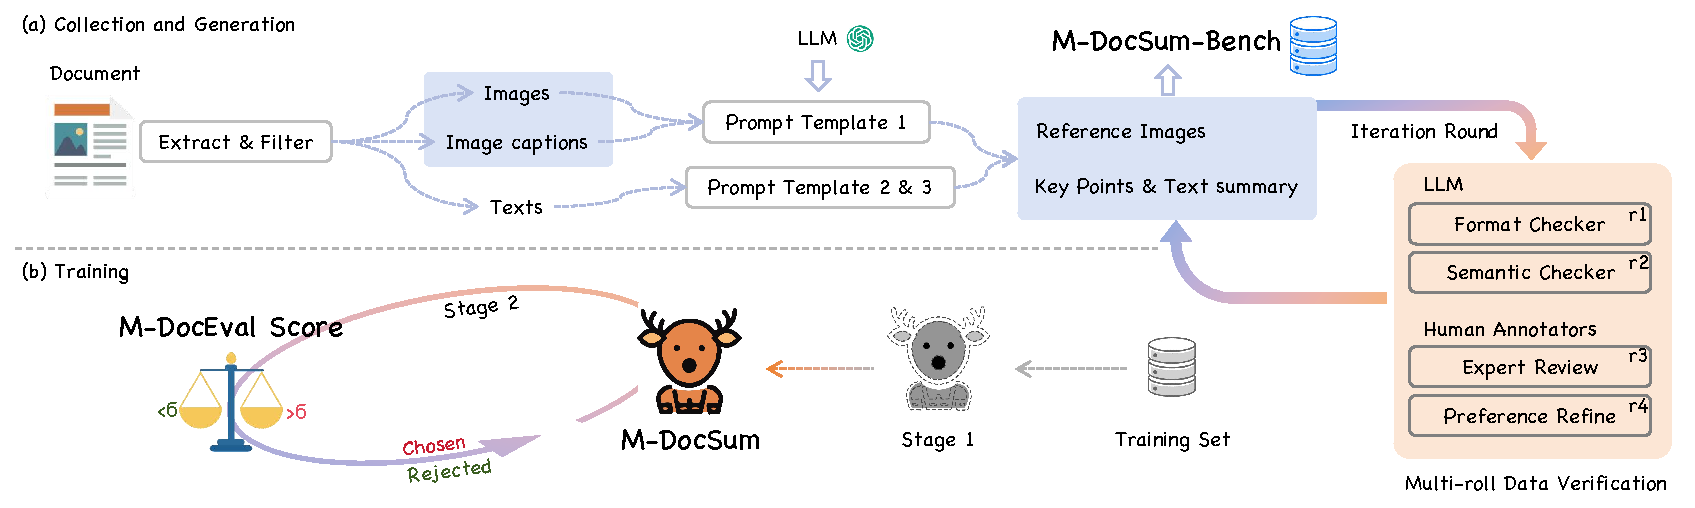
\includegraphics[width=\textwidth]{figs/fig_main}
\caption{The illustration of automated data construction pipeline, multi-roll data verification, and two-stage training.}
\label{fig-main}
\end{figure*}

\subsection{Task Define}
We introduce the M-DocSum task, given the extensive demand for comprehending and summarizing lengthy documents such as scientific articles and technical reports, we have selected scientific articles from arXiv.
The input comprises two modalities, first, the textual information of the scientific article is parsed into complex markdown format, preserving not only the main body of the text but also critical elements like tables and image captions. 
Second, the accompanying images within the article are parsed into image format, retaining their original visual information. 
These two modalities are then fed into the model in an interleaved manner, simulating the natural alternating text-image experience of human readers when engaging with scientific articles. 
Following model processing, a structured output is generated, including: 1) Summary text: a concise summary of the article's core content divided into four fixed paragraphs, covering essential information such as background, main arguments, experimental results or analysis, and conclusions. 
2) Referenced images: the model generates indices for referenced images along with their corresponding captions. The captions show the reasoning when making the selection.
By matching these indices with the original image sequence, we parse the output into the final interleaved summary format. 
This output format not only demands strong text summarization skills from the model but also requires accurate identification and referencing of key images, demonstrating a comprehensive understanding of multimodal information. 
Additionally, the fixed paragraph structure provides clear criteria for evaluating the generation, facilitating both automated and human assessments.


\subsection{Dataset Collection}
\label{sec:3.2}
To support our evaluation benchmark, we process high-quality multimodal documents from the publicly accessible arXiv website~\footnote{\url{https://arxiv.org/}}~\cite{he2024pasa},
primarily focusing on six domains: Artificial Intelligence, and AI-related fields such as Engineering, Computer Science, Physics, Mathematics, and Medicine, given the specialized knowledge required for academic articles. 
To mitigate the risk of data contamination or memorization by existing models, we limit the publication dates to April 2024 or later. 
We filter out documents without images and those exceeding 32k text tokens, ultimately collecting 4.2k high-quality academic articles. 
We carefully select 500 articles for the M-DocSum-Bench for broader benchmark coverage, reserving the remaining 3.7k documents for the training set. 
We have taken steps to ensure the integrity and accuracy of the multimodal data within this benchmark.  
For the evaluation, the images contained within the M-DocSum-Bench are considered authoritative.
As shown in Table~\ref{tab:statis} and Figure~\ref{fig:1_statisticians}, we compile detailed basic information, including document length, number of images, and the proportion of each subject. 
The collection of this data lays the foundation for subsequent exploration of the performance of LVLMs.


\subsection{Interleaved Summary Generation}
\label{sec:3.3}
As shown in Figure~\ref{fig-main}(a), to create a high-quality benchmark, we design a meticulous automated framework for generating summary texts and selecting referenced images. 
Initially, we extract key points for each summary paragraph from the original text, adhering to specific rules: ensuring no repetition of information, maintaining atomicity so each point is an independent, indivisible unit, verifying that each point is traceable back to the original text, and limiting the number of key points per paragraph to no more than 10. 
Once these key points are confirmed, we utilize advanced LLM like GPT-4o to synthesize them into coherent and comprehensive paragraph summaries.

For image referencing, we provide the extracted key points, original images, and image captions to a powerful LVLM.
The model first determines if an image is necessary to aid understanding of the summary paragraph. 
If deemed necessary, it selects the most suitable image based on criteria such as high relevance to the paragraph's content, providing crucial visual support that complements textual information, and ensuring that only one image is referenced per paragraph and each image is used only once. 
Detailed descriptions of our selection and generation processes are available in Appendix Figure~\ref{fig:prompt1},~\ref{fig:prompt2}, and~\ref{fig:prompt3}.


\subsection{Quality Control}
\label{sec:3.4}
As shown in Figure~\ref{fig-main}(right), we introduce Multi-roll Data Verification, a semi-automatic quality control process combining LLMs and human expertise to ensure high benchmark quality. 
Initially, LLMs perform two rounds of validation: Round 1 checks for necessary key fields and at least one image reference in the summary format, while Round 2 ensures semantic integrity by identifying repetitive or invalid content. 
Summaries failing these checks are iteratively regenerated. 
Following LLM validation, domain experts conduct thorough reviews, spending at least 20 minutes on each document to correct any hallucinations or semantic distortions. 
They also refine image references to align with human reading habits. 
Additionally, annotators cross-check each other’s work, with primary reviewer resolving any disagreements to maintain consistency. 
This rigorous process ensures a high-quality, reliable benchmark for advancing multimodal document understanding.

\subsection{M-DocEval}
\label{sec:3.5}
To provide a comprehensive and objective assessment of the performance in generating interleaved summaries, we design a multifaceted set of evaluation metrics. 
These metrics cover textual quality, image referencing appropriateness, and instruction-following capability, ensuring a holistic evaluation of the model abilities.
Specific details regarding text and image reference evaluation can be found in Appendices Figure~\ref{fig:case_en_2} and~\ref{fig:case_en_1}.

\textbf{Textual Content Evaluation.} The text summary evaluation focuses on two primary aspects:
(1) Completeness~(Com) measures the proportion of essential information captured from the original text using a benchmark set of key points, generated and verified by human experts. 
(2) Accuracy~(Acc) assesses the correctness of the summary by comparing each sentence to the original content, rewarding matches and penalizing hallucinations, repetitions, or semantic distortions. 
We compute the Text Score~(TS) as the F1 score of completeness and accuracy:
\begin{equation}
\text{TS} = \frac{2 * \text{Com} * \text{Acc}}{\text{Com} + \text{Acc}}.
\end{equation}
This balanced score ensures a comprehensive assessment of the textual quality.
Specific prompt details can be found in Appendix Figure~\ref{fig:prompt_com} and ~\ref{fig:prompt_acc}.

\textbf{Visual Reference Evaluation.} For image referencing, we evaluate the model's ability to determine image necessity and select appropriate images correctly. 
(1) None Accuracy~(NonAcc) assesses the correct identification of paragraphs needing no image. 
(2) Image Accuracy~(ImgAcc) measures precise image matching for paragraphs requiring images. 
(3) Overall Matching Rate~(OMatch) provides an overall assessment of correct image decisions across all paragraphs. 
(4) Jaccard Similarity~(JacSim) evaluates the similarity between the model's referenced images and the correct set, excluding ``None" cases, offering insight into image selection accuracy regardless of placement. 
The Image Score~(IS) is computed as the weighted average of Overall Matching Rate and Jaccard Similarity:
\begin{equation}
\text{IS} = \frac{\text{OMatch} + \text{JacSim}}{2}.
\end{equation}
This score reflects both the correctness of image selection and the overall appropriateness of image references in the summary, ensuring a robust and objective evaluation framework.

\textbf{Instruction Following Capability.} Given that open-source multimodal models may not always generate content that fully adheres to the given instructions, we introduce an Instruction Following Capability~(IF) metric. 
This metric evaluates how well the model follows instructions by assessing whether it produces appropriate summary texts and image references as specified.

To obtain a final, comprehensive evaluation of each sample, we integrate the TS, IS, and IF using a weighted average:
\begin{equation}
    Total = \alpha * IF + \beta * TS + \gamma * IS,
\end{equation}
where $\alpha, \beta, \gamma$ are $0.1, 0.45, 0.45$, respectively. This weighting scheme ensures that while instruction adherence is important, the quality of the textual and visual content remains the primary focus.